\documentclass[conference]{IEEEtran}

% Swedish language package 
\usepackage[utf8]{inputenc}
\usepackage[T1]{fontenc}
\usepackage[english]{babel}

% Graphics
\usepackage{graphicx, float, subfigure, blindtext}

\newcommand\IEEEhyperrefsetup{
bookmarks=true,bookmarksnumbered=true,%
colorlinks=true,linkcolor={black},citecolor={black},urlcolor={black}%
}

% Preferred hyperref setup, Michael Shell
\usepackage[\IEEEhyperrefsetup, pdftex]{hyperref}

% Maths
\usepackage{mathtools}

% These packages must be at the end
\usepackage[nolist,nohyperlinks]{acronym}
\usepackage{cleveref}
\graphicspath{{images/}}

% Remove section first paragraph indent
\usepackage{titlesec}
\titlespacing*{\section}{0pt}{*1}{*1}
\titlespacing*{\subsection}{0pt}{*1}{*1}
\renewcommand{\thesubsubsection}{\arabic{subsubsection}}
\titleformat{\subsubsection}[runin]{\itshape}{\thesubsubsection)}{1em}{}[:]
\titlespacing*{\subsubsection}{\parindent}{0pt}{*1}

% Include authors 
\author{\IEEEauthorblockN{}
\IEEEauthorblockA{
Kai-Po Lin\\
Email: kl72@rice.edu
}}

% The report title.
\title{The 3D-sensing technologies of Autonomous Navigation and Metaverse}
% Document begins here
\begin{document}
% Create the title.
\maketitle
% Example sections, name them
% according to specific needs.
\begin{abstract}
Autonomous navigation and metaverse are doubly two of the promising areas that benefit hugely to our human beings. With the help of autonomous navigation, we can let the system come up with the fastest route to safely and effortlessly drive us to our destination. While with the help of the metaverse, we can virtually go to many places we want without traveling and the limit of the space capacity. In this paper, I would like to introduce these two technologies, comparing their 3D-sensing tech specs and the challenges they are facing, then talk about their potentials and future trends.
\end{abstract}
\section{Introduction}
Before talking about the main 3D-sensing techniques of autonomous navigation and metaverse, let’s talk about their history:

Autonomous Navigation \cite{autonomousHistory} — In the 1500 centuries before the invention of any modern technology, Leonardo da Vinci designed a cart, which is considered the world’s first robot that could move without being pushed or pulled. Years later in 1933, the demand for extended travel times forced the development of autopilot systems for long-range aircraft. Mechanical Mike was a prototype autopilot designed by Sperry Gyroscope Co. and used by Wiley Post during a 13,000-mile, around-the-world flight. In 1961, a Stanford engineering graduate student James Adams develop the world’s first truly self-driving wheeled vehicle, which was eventually outfitted with cameras and programmed to detect and autonomously follow a solid white line on the ground. And eventually, the most well-known Tesla autonomous driving car was introduced in late 2015.

\begin{figure}[H]
    \centering
    \subfigure{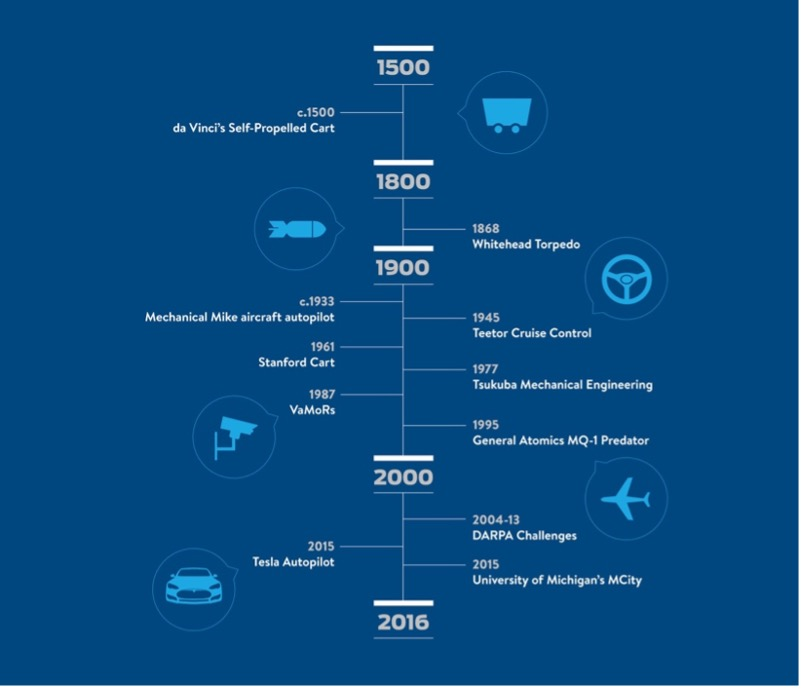
\includegraphics[width=.791\columnwidth]{autoHis}}
    \caption[Short text]{The history of Autonomous Navigation \cite{autonomousHistory}}
    \label{fig:autoHis}
\end{figure}

Metaverse \cite{metaverseHistory} — The term “metaverse” first comes from a sci-fi writer Neal Stephenson in 1992, to describe a 3D virtual space. While currently, the word “metaverse” is a digital world created by the infusion of different technologies like Virtual Reality (VR), Augmented Reality (AR), and the Internet. The most famous applications nowadays are Philip Rosedale's “Second Life” online virtual world in 2003 and Mark Zuckerberg's 2021 announcement of Meta's metaverse plan.

\begin{figure}[H]
    \centering
    \subfigure{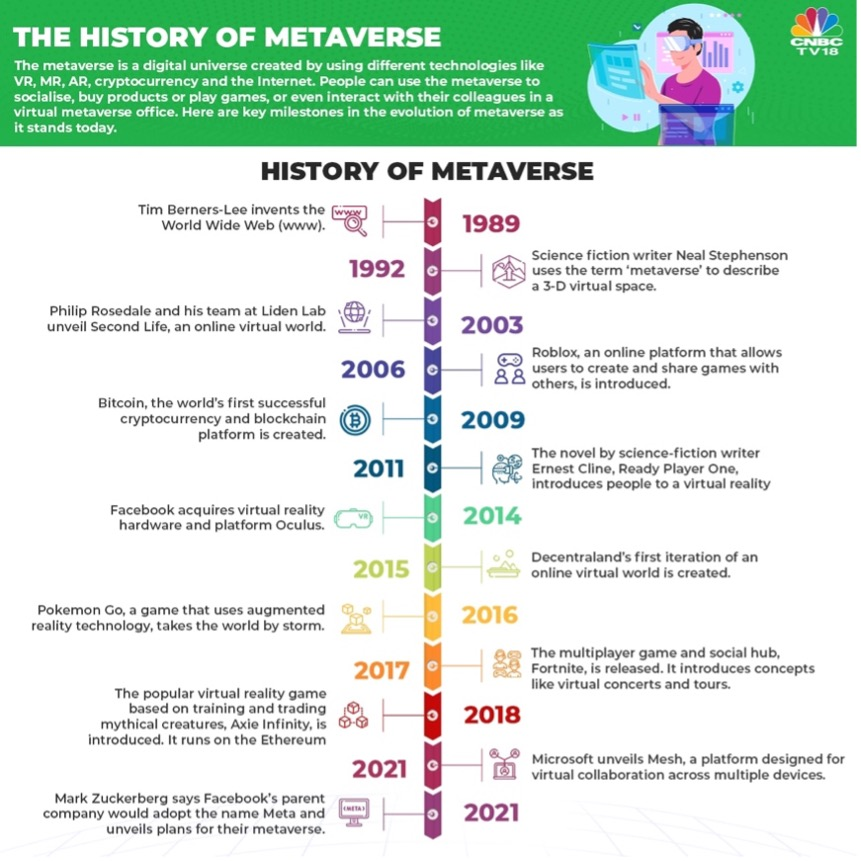
\includegraphics[width=.791\columnwidth]{metaverseHis}}
    \caption[Short text]{The history of Metaverse \cite{metaverseHistory}}
    \label{fig:metaverseHis}
\end{figure}
\section{Techniques Comparison}
\label{section:techniques}
Here is the comparison of the 3D-sensing techniques between autonomous navigation and the metaverse:
\\\\
\textbf{1.	Autonomous Navigation}
\\\\
The 3D-sensing techniques of Autonomous navigation is composed with \textbf{cameras, Radar, Ultrasound, IMU, and LiDAR sensors} surrounded around the car to simulate the actual environment beside the car.
\begin{figure}[H]
    \centering
    \subfigure{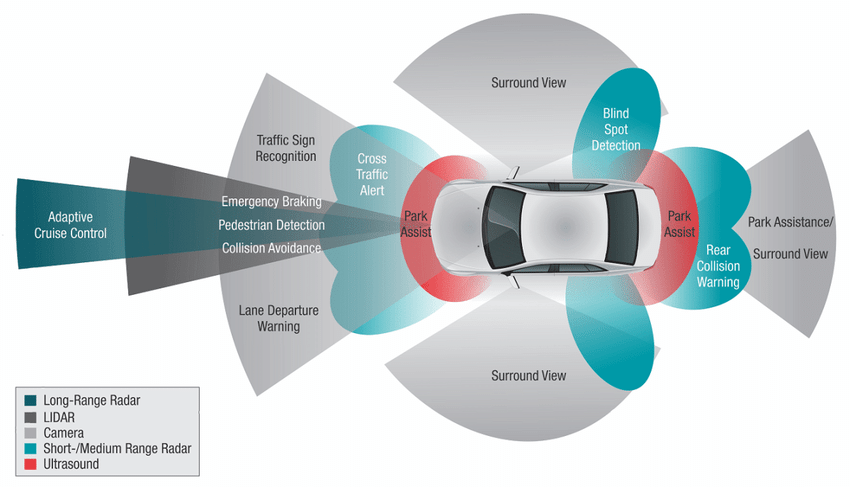
\includegraphics[width=.9\columnwidth]{images/Camera.png}}
    \caption[Short text]{3D-sensors in autonomous navigation \cite{autonomousPic}}
    \label{fig:Camera}
\end{figure}

(1)	\textbf{Camera} \cite{autonomousSensor}: To obtain 3D-colored images, at least two cameras are required.
\\\\
(2)	\textbf{Radar} \cite{autonomousSensor}: In recent decades they have also been installed in vehicles to measure distances to obtain reliable data for systems such as the spacer and the emergency brake assistant, regardless of weather conditions. The sensors emit short pulses in the form of electromagnetic waves (radio waves), which are propagated almost at the speed of light. As soon as the waves hit an object, they are reflected and bounce back to the sensor. The shorter the time interval between transmission and reception, the closer the object is. This technology enables the use of driver assistance systems such as adaptive cruise control and collision avoidance.
\\\\
(3)	\textbf{Ultrasound} \cite{autonomousSensor}: Ultrasound is used for the closed range danger detection (limited to less than 10 meters); it can detect the full surrounding of a car within a short-range. Ultrasound is mainly used for parking aid, monitoring the blind spot, and for emergency brake assistants. It is based on the time-of-flight principle, which emitted sound waves at a frequency of 20,000 Hz.
\\\\
(4)	\textbf{IMU} \cite{ARIMU} \cite{autonomousIMU}: The IMU provides information on current vehicle location and orientation. An IMU combines three types of sensors: an accelerometer, a gyroscope, and a magnetometer. The accelerometer measures linear acceleration, the gyroscope measures rotational acceleration, and the magnetometer is a device capable of measuring magnetism, which can help us find orientation using the earth's magnetic field, like a compass. Each of these sensing elements must also sense the measured property in 3 axes, (X, Y, Z). Each sensor employs a fabrication technology known as “MEMS”, Micro-Electro-Mechanical Systems. This fabrication technology is based on Integrated Circuit Photolithography techniques.
\\\\
(5)	\textbf{LiDAR} \cite{autonomousSensor}: In contrast to ultrasonic sensors, LiDAR sensors are suitable for both short- and long-range use. Although they have existed for many years, they have only been used increasingly in vehicles since the 2000s. LiDAR is considered a key technology for achieving higher levels of autonomy because they measure the distance of objects at incredible speeds and with high precision. LiDAR sensors emit up to one million laser pulses per second and summarize the results in a high-resolution 3D map of the environment.
\\\\
\textbf{2.	Metaverse}
\\\\
Metaverse combines the techniques of \textbf{Virtual Reality (VR), Augmented Reality (AR)}, and \textbf{the Internet}. As for AR \cite{metaverseSensor}, to augment our reality, the system must first understand exactly what reality it is they are working with. That is, both \textbf{camera} and \textbf{LiDAR} will be the best tool to quantify the spaces in our lives. \cite{ARIMU} Moreover, for a VR headset system to accurately adjust the projected image on the viewscreen, or an AR system to place the projected holographs, the computer must know the relative location and motion of the wearer’s head. An \textbf{Inertial Measurement Unit (IMU)} is typically used to accomplish this task.
\\\\
(1)	\textbf{Camera and LiDAR}: Used for environment simulation. Also used in the 3D-sensing of autonomous navigation.
\\\\
(2)	\textbf{Inertial Measurement Unit (IMU)}: Combining these signals facilitates error correction and yields accurate measurements to track head position and movement. Also used in the 3D-sensing of autonomous navigation.
\\\\
\textbf{In conclusion}, Metaverse uses Camera, LiDAR, and IMU to keep track of the user’s information as well as to simulate the environment. Similarly, autonomous navigation also takes advantage of Camera, LiDAR, and IMU to gather the car’s position and environmental information; however, since autonomous navigation requires more information to alert the driver and to make a decision, it obsesses more sensors like Ultrasound and Radar to support the whole system.
\section{Challenges}
\label{section:challenges}
\textbf{Autonomous Navigation}

One of the most difficult problems for autonomous navigation is that it must explore and keep track of the environment in real-time. Most importantly, we must make sure that autonomous navigation rarely makes mistakes since accidents might occur if any part of the hardware or software system encounters a single error. Perhaps a single parameter that was overweighted in a system may cause serious accidents.

Moreover, some researchers also debated that the system would face a dilemma when it encounters some ethical or psychological problems such as the Trolley Problem. That is, even if the autonomous navigation system is functional and did help the driver to save plenty of effort, it is still now served as a role of auxiliary instead of the driver.
\\\\
\textbf{Metaverse}

Metaverse has several challenges to overcome \cite{metaverseChallenge}, such as how to identify who the person is (which may further cause security problem) or lack of clarifying laws to protect and follow.

First, it is extremely essential to figure out how to prove who you are in virtual reality, instead of another person or even a bot trying to mimic your existence. This will require building new methods of personal data and privacy protection that will be able to ensure the safety of one’s identity and possessions in the virtual world. In other words, personal verification might come to the point where users will have to provide more personal data than what is expected today, to identify themselves and ensure the security system works efficiently, keeping personal data safe.

Finally, Metaverse is bound to bring large numbers of users together, making it a place of great opportunity to connect and exchange, however at the same time making users vulnerable in case there are no laws that regulate the boundaries. It will be a true challenge to identify jurisdiction as well as set legislation that can ensure the virtual space is safe and secure for its users.
\section{Future Trends}
Finally, let's discuss all the potential future trends of Autonomous Navigation and Metaverse:
\\\\
1.	Autonomous Navigation \cite{autonomousFuture}
\\\\
(1)	Ability to Learn Driver’s Routines and Preferences

Driverless cars can leverage their machine learning capabilities to learn the routines and preferences of their passengers. For example, providing greater assistance by automatically performing routine tasks such as ensuring on-time arrival for work or appointments, finding a cheap parking spot in dense cities, or preferentially driving to stores where specific, desired products are in stock.
\\\\
(2) Enhance Driving Safety

After solving the challenges of autonomous navigation. We can soon arrive at our destination by choosing the fastest and safest route.
\\\\
(3)	In-Vehicle Advertising

Advertising will be a big part of the experience at some point. While on the way to your destination, you’ll be able to add a stop for shopping or food, and companies will be vying for that recommendation. Briefly, you’ll be able to see the extra time needed and be able to order in transit.
\\\\
(4)	Better Privacy and Cybersecurity Features

Future driverless cars will \textbf{incorporate more privacy and security features}. Firewalls in cars will be normalized. Protection of the driver’s data will become paramount, and it will likely be regulated.
\\\\
(5)	Multi-Internet Communications Systems

Future driverless cars will be able to communicate with each other as well as with retailers and restaurants, enabling curbside and drive-through pickups. Authorized e-commerce companies will be able to access and deliver items directly to the vehicle’s trunk.
\\\\
2.	Metaverse
\\\\
(1)	New Mode for Online Shopping \cite{metaverseFuture1}

\textbf{Consumers will no longer need to frequent physical stores to try new products before purchasing}. VR and AR experiences will allow exploration of brands and their offerings from the comfort of customers’ homes. On the other hand, the metaverse will also enable more interactive in-store experiences.
\\\\
(2)	Own and Trade Properties in Metaverse \cite{metaverseFuture2}

\textbf{Once you own something in the metaverse, it can be sold or traded to one of the other users}. This adds an element of wealth and prestige to an otherwise detached world. Some lots are worth more than others, some items are rare while others are common — all of this adds up to the creation of an economy that applies to a particular metaverse.
\\\\
(3)	Changing How We Live and Interact \cite{metaverseFuture2}

Metaverse can become \textbf{a place almost capable of replacing reality}. We’re not quite there yet (and we won’t be for years), but the efforts of companies like Meta or VRChat are bringing us closer to this than we’ve ever been before. In a perfect metaverse, you can interact with every person around you and perhaps work, study, meet friends, or even form a study group in a virtual library inside the metaverse.
\section{Conclusion}

To sum up, both autonomous navigation and metaverse use plenty of 3D-sensors, such as LiDAR, Camera, and IMU to perceive and simulate their surroundings. However, \textbf{autonomous navigation requires more additional sensors} like Ultrasound and Radar to help the driver keep away from danger and gather more information to help the system better make up decisions.
% Select the IEEEtran style
\bibliographystyle{IEEEtran}
% Include bibliography file
\bibliography{IEEEabrv,refs}
\end{document}